
\documentclass[11pt,halfline,a4paper,]{ouparticle}

% Packages I think are necessary for basic Rmarkdown functionality
\usepackage{hyperref}
\usepackage{graphicx}
\usepackage{listings}
\usepackage{xcolor}
\usepackage{fancyvrb}
\usepackage{framed}

% Link coloring
\hypersetup{breaklinks=true,
            bookmarks=true,
            pdfauthor={},
            pdftitle={Revisiting the Measurement and Dimensionality of Political Knowledge: Evidence from Seven European Countries}
            }


% For knitr::kable functionality
\usepackage{booktabs}
\usepackage{longtable}

%% To allow better options for figure placement
%\usepackage{float}

% Packages that are supposedly required by OUP sty file
\usepackage{amssymb, amsmath, geometry, amsfonts, verbatim, endnotes, setspace}

% For code highlighting I think
\DefineVerbatimEnvironment{Highlighting}{Verbatim}{commandchars=\\\{\}}
\definecolor{shadecolor}{RGB}{248,248,248}
\newenvironment{Shaded}{\begin{snugshade}}{\end{snugshade}}
\newcommand{\AlertTok}[1]{\textcolor[rgb]{0.94,0.16,0.16}{#1}}
\newcommand{\AnnotationTok}[1]{\textcolor[rgb]{0.56,0.35,0.01}{\textbf{\textit{#1}}}}
\newcommand{\AttributeTok}[1]{\textcolor[rgb]{0.77,0.63,0.00}{#1}}
\newcommand{\BaseNTok}[1]{\textcolor[rgb]{0.00,0.00,0.81}{#1}}
\newcommand{\BuiltInTok}[1]{#1}
\newcommand{\CharTok}[1]{\textcolor[rgb]{0.31,0.60,0.02}{#1}}
\newcommand{\CommentTok}[1]{\textcolor[rgb]{0.56,0.35,0.01}{\textit{#1}}}
\newcommand{\CommentVarTok}[1]{\textcolor[rgb]{0.56,0.35,0.01}{\textbf{\textit{#1}}}}
\newcommand{\ConstantTok}[1]{\textcolor[rgb]{0.00,0.00,0.00}{#1}}
\newcommand{\ControlFlowTok}[1]{\textcolor[rgb]{0.13,0.29,0.53}{\textbf{#1}}}
\newcommand{\DataTypeTok}[1]{\textcolor[rgb]{0.13,0.29,0.53}{#1}}
\newcommand{\DecValTok}[1]{\textcolor[rgb]{0.00,0.00,0.81}{#1}}
\newcommand{\DocumentationTok}[1]{\textcolor[rgb]{0.56,0.35,0.01}{\textbf{\textit{#1}}}}
\newcommand{\ErrorTok}[1]{\textcolor[rgb]{0.64,0.00,0.00}{\textbf{#1}}}
\newcommand{\ExtensionTok}[1]{#1}
\newcommand{\FloatTok}[1]{\textcolor[rgb]{0.00,0.00,0.81}{#1}}
\newcommand{\FunctionTok}[1]{\textcolor[rgb]{0.00,0.00,0.00}{#1}}
\newcommand{\ImportTok}[1]{#1}
\newcommand{\InformationTok}[1]{\textcolor[rgb]{0.56,0.35,0.01}{\textbf{\textit{#1}}}}
\newcommand{\KeywordTok}[1]{\textcolor[rgb]{0.13,0.29,0.53}{\textbf{#1}}}
\newcommand{\NormalTok}[1]{#1}
\newcommand{\OperatorTok}[1]{\textcolor[rgb]{0.81,0.36,0.00}{\textbf{#1}}}
\newcommand{\OtherTok}[1]{\textcolor[rgb]{0.56,0.35,0.01}{#1}}
\newcommand{\PreprocessorTok}[1]{\textcolor[rgb]{0.56,0.35,0.01}{\textit{#1}}}
\newcommand{\RegionMarkerTok}[1]{#1}
\newcommand{\SpecialCharTok}[1]{\textcolor[rgb]{0.00,0.00,0.00}{#1}}
\newcommand{\SpecialStringTok}[1]{\textcolor[rgb]{0.31,0.60,0.02}{#1}}
\newcommand{\StringTok}[1]{\textcolor[rgb]{0.31,0.60,0.02}{#1}}
\newcommand{\VariableTok}[1]{\textcolor[rgb]{0.00,0.00,0.00}{#1}}
\newcommand{\VerbatimStringTok}[1]{\textcolor[rgb]{0.31,0.60,0.02}{#1}}
\newcommand{\WarningTok}[1]{\textcolor[rgb]{0.56,0.35,0.01}{\textbf{\textit{#1}}}}

% use upquote if available, for straight quotes in verbatim environments
\IfFileExists{upquote.sty}{\usepackage{upquote}}{}

% For making Rmarkdown lists
\providecommand{\tightlist}{%
  \setlength{\itemsep}{0pt}\setlength{\parskip}{0pt}}

% Macros for dealing with affiliations, footnotes, etc.
\makeatletter
\def\Newlabel#1#2#3{\expandafter\gdef\csname #1@#2\endcsname{#3}}

\def\Ref#1#2{\@ifundefined{#1@#2}{???}{\csname #1@#2\endcsname}}

\newcommand*\samethanks[1][\value{footnote}]{\footnotemark[#1]}

\newcommand*\ifcounter[1]{%
  \ifcsname c@#1\endcsname
    \expandafter\@firstoftwo
  \else
    \expandafter\@secondoftwo
  \fi
}

\newcommand*\thanksbycode[1]{%
  \ifcounter{FNCT@#1}
    {\samethanks[\value{FNCT@#1}]}
    {\thanks{\Ref{FN}{#1}}\newcounter{FNCT@#1}\setcounter{FNCT@#1}{\value{footnote}}}
}

% Create labels for Addresses if the are given in Elsevier format

% Create labels for Footnotes if the are given in Elsevier format
\Newlabel{FN}{1}{Current email address:
\href{mailto:cat@example.com}{cat@example.com}.}

% Part for setting citation format package: natbib

% Part for setting citation format package: biblatex

% Part for indenting CSL refs
% Pandoc citation processing
% Pandoc header
\usepackage{booktabs}
\usepackage{longtable}
\usepackage{array}
\usepackage{multirow}
\usepackage{wrapfig}
\usepackage{float}
\usepackage{colortbl}
\usepackage{pdflscape}
\usepackage{tabu}
\usepackage{threeparttable}
\usepackage{threeparttablex}
\usepackage[normalem]{ulem}
\usepackage{makecell}
\usepackage{xcolor}

\begin{document}

\title{Revisiting the Measurement and Dimensionality of Political
Knowledge: Evidence from Seven European Countries}

\author{%
%
% Code for old style authors field
%
% Add \and if both authors and author
%
%
% Code for new (elsevier) style author field
\name{William Allen}
%
\email{\href{mailto:william.allen@politics.ox.ac.uk}{william.allen@politics.ox.ac.uk}}%
\thanks{Corresponding author; Email: \href{mailto:william.allen@politics.ox.ac.uk}{william.allen@politics.ox.ac.uk}}%
%
%
\and
\name{Kristoffer Ahlstrom-Vij}
%
\email{\href{mailto:k.ahlstrom-vij@bbk.ac.uk}{k.ahlstrom-vij@bbk.ac.uk}}%
%
%
%
%
}

\abstract{Knowledge matters for the political preferences people form,
and the choices they make. Despite the recent growth of experimental
work, however, the bulk of research on political knowledge still uses
observational data, where researchers typically rely on batteries of
general political knowledge questions to distinguish more from less
informed voters. When used to explain outcomes across policy-specific
domains, this practice invokes what we call a generalist assumption:
possessing general knowledge is diagnostic of holding issue-specific
knowledge (and vice versa). As the list of geographical areas and issue
domains of interest to political scientists grow, the weight put on this
assumption increases significantly; so, is it warranted? Using 2018
survey data from seven European countries (Germany, Hungary, Poland,
Romania, Spain, Sweden, and the UK) that, unusually, includes knowledge
questions about both general politics as well as about EU immigration (N
= 10,749), we combine several approaches to test the core expectations
of the generalist assumption: First, exploratory and confirmatory factor
analyses suggest that the combined set of questions is plausibly
unidimensional. Second, after constructing Item Response Theory (IRT)
knowledge scales from the items, we demonstrate how both scales display
similar associations with key respondent features -- gender, age, and
education -- known to be correlated with political knowledge, and also
with two reference sets containing established measures of general
political knowledge from BES and ANES, including when broken down by
country. Finally, we show that the estimated marginal mean level of
general political as well as immigration knowledge by aforementioned
respondent features exhibit similar patterns with independent scales
measuring knowledge on public health and climate change, suggesting that
the evidence from the previous steps was not an artefact of immigration
knowledge being a unique case. We conclude that the preponderance of
evidence points to the generalist assumption standing up to scrutiny.
However, we caution against deploying it uncritically and offer our code
as a means of enabling others to conduct similar stress-tests.}

\date{\today}

\keywords{political knowledge; immigration; public health; climate
change}

\maketitle



\hypertarget{introduction}{%
\section{Introduction}\label{introduction}}

Knowledge matters for politics, and yet citizens are generally un- or
misinformed about poliitcal matters (Fowler and Margolis 2014). This
presents a problem not only for the integrity of their political voice
but also for representation: If an electorate making choices based on
false beliefs is more likely to express political preferences that they
might not have held, had they been more informed, then when political
representatives cater to the public's stated preferences, the people
expressing those preferences are not well-represented (Bartels 1996;
Delli Carpini and Keeter 1996). Indeed, as a cognitive division of
labour is at the very heart of representative democracy, representatives
who uncritically mirror the political voices of the represented run the
risk of operating in bad faith.

For these reasons, political scientists are rightly concerned with the
relationship between knowledge and political opinion (Kuklinski et
al.~2000; Munger et al.~2020). A growing body of work -- largely
experimental in nature -- has demonstrated how citizens across diverse
contexts respond to factual interventions in predictable ways (Walter et
al.~2020), notably by moving their beliefs towards more factually
correct positions (Carnahan and Bergan 2021; Guess and Coppock 2018;
Porter and Wood 2021). Yet existing evidence on whether and to what
extent such knowledge shifts attitudes and preferences in particular
directions is less clear, particularly when it comes to specific issues
such as immigration which evoke strong partisan cleavages (Blinder and
Schaffner 2019; Grigorieff, Roth, and Ubfal 2020; Hopkins, Sides, and
Citrin 2018).

Moreover, bespoke experimental designs, while highly internally valid,
are often not an option for many researchers and projects due to
resource constraints, especially for large-scale, comparative
investigations. What follows therefore draws on parallel developments in
information effects research which typically uses existing observational
data to model to what extent holding different levels of knowledge
matter for political behaviours, including vote choice (Bartels 1996;
Blais et al.~2009; Delli Carpini and Keeter 1996; Oscarsson 2007) as
well as preferences and attitudes on specific issues (Althaus 2003;
Ahlstrom-Vij 2021). However, political attitudes encompass a wide range
of specific issues: immigration, climate, welfare, foreign policy, to
name but a few. In order to make judgments about the role of information
across such domains, an assumption is typically made in the information
effects literature: people who are knowledgeable in one area of politics
will be knowledgeable in others as well (e.g., Zaller 1986 and 1992;
Delli Carpini and Keeter 1996). We call this the generalist assumption.

The attraction of that assumption should be obvious: if it holds,
researchers can use a general knowledge scale to measure the extent to
which people are politically informed across specific domains, even in
the absence of items directly concerned with the particular topics
represented within those domains. Yet, despite its methodological
centrality, this assumption has remained largely untested (although see
Delli Carpini and Keeter 1996 for an early exception that we will be
returning to below), partly due to the lack of available survey
instruments which contain both general and issue-specific factual items.
In response, we present analysis using data from a cross-national
European survey that, unusually, contains data on respondents' knowledge
both about general politics and on a specific issue -- in this case,
immigration -- as well as their attitudes on that issue (Meltzer et
al.~2019). By applying several methods to assess the dimensionality and
construct validity of these different types of knowledge questions, and
by comparing the resulting scales to a variety of other instruments, we
conclude that the generalist assumption is defensible but should not be
invoked uncritically. Instead, researchers using available knowledge
questions on observational surveys would be well-served by
stress-testing their conclusions using other data where available.
Finally, in line with Open Science principles, we publicly offer our
approach (its code and method) as a template for others.\footnote{See
  https://github.com/ahlstromvij/REMINDER\_project. More broadly, we
  hope our approach enables other researchers to replicate our analyses
  for their own purposes in so far as they either (a) have data sets
  with different knowledge items and want to evaluate for dimensionality
  in order to decide on what scale to use; or (b) are collecting data
  and want to run a pilot with different items, use our approach, and
  then potentially save funds and time (and respond to quality concerns
  relating to survey attentiveness) on only collecting on the items that
  this analysis suggests that they need (e.g.~by skipping domain
  specific items if not needed).}

\hypertarget{the-generalist-assumption-about-political-knowledge}{%
\section{The Generalist Assumption about Political
Knowledge}\label{the-generalist-assumption-about-political-knowledge}}

The generalist assumption can be traced back at least to John Zaller's
analysis of information items in the 1985 National Election Study Pilot,
where he argued that ``political information is a relatively general
trait that can be effectively measured with a general-purpose
information scale'' (Zaller 1986, 2). This conclusion subsequently
informed his landmark study on public opinion, where he noted that he
was ``assuming that persons who are knowledgeable about politics in
general are habitually attentive to communications on most particular
issues as well'' (Zaller 1992, 43). That same assumption is investigated
and defended by Delli Carpini and Keeter (1996), and relied upon in both
Bartels's (1996) and Althaus's (2003) highly influential work on
information effects, measuring differences between actual preference
reports and modeled estimates of the preferences reports respondents
likely would have given, had they been fully informed.

In operationalizing the relevant notion of informedness, Bartels relies
upon interviewer ratings of respondents' ``general level of information
about politics and public affairs'' (1996, 203) while Althaus uses the
type of general scales developed by Delli Carpini and Keeter. Subsequent
work across a variety of geographical contexts including the US
(Ahlstrom-Vij 2021), Denmark (Bhatti 2010; Hansen 2009), Sweden
(Oscarsson 2007) and Canada (Blais et al.~2009) follows the norms set by
these early studies by using either a variety of general knowledge items
or a scale of both general and specific campaign items alongside
interviewer ratings of the respondent's knowledge. As such, the
generalist assumption has come to carry an increasingly heavy burden:
not only is the catalogue of geographical contexts in which researchers
investigate the impacts of knowledge on political attitudes and choice
expanding, but so also is the list of the specific political and policy
issues that feature either directly or indirectly in models of voter
attitude and choice in a range of political circumstances.

In parallell, there has been a growth in experimental work on the role
of knowledge and information on specific policy matters, one such area
being immigration. For example, providing corrective information about
the levels and impacts of immigration appears to reduce misconceptions
and change attitudes (Grigorieff, Roth, and Ubfal 2020), as well as
policy preferences in some circumstances (Blinder and Schaffner 2019;
Facchini, Margalit, and Nakata 2022), although the presence and
direction of these effects is not consistent (Jørgensen and Osmundsen
2020). Clearly, further work is needed, but due to resource constraints,
much of that research will need to be observational rather than
experimental, in which case researchers will in many cases need to rely
on available general knowledge items even when concerned with specific
policies issues. This puts further pressure on the generalist
assumption.

So, does that assumption hold? That is the question we set out to answer
below, using immigration knowledge and general political knowledge as
our test case, before moving on to a wider set of issue-specific
knowledge scales. If the assumption holds, we expect that different
methods of analysis (which we describe later) will converge to support
its core expectations: that (1) relevant pattern of observed variables
can plausibly be represented by a single latent trait (factor) in factor
analysis; (2) regressing the knowledge scales on demographic variables
will produce associations that one would expect from prior work into the
determinants of political knowledge, where those associations will both
be in line with patterns found in established measures of political
knowledge from BES and ANES, and hold cross-nationally; and (3) the
estimated marginal mean level of general political knowledge by
education, gender, and age should exhibit the same pattern not only on
the two scales above, but also on independent scales measuring knowledge
on other, issue-specific matters, namely: public health and climate
change.

\hypertarget{methods-and-data}{%
\section{Methods and Data}\label{methods-and-data}}

\hypertarget{dataset}{%
\subsection{Dataset}\label{dataset}}

We use a subset of online survey data collected as part of the REMINDER
(Role of European Mobility and Its Impacts in Narratives, Debates and EU
Reforms) project (Meltzer et al.~2019).\footnote{Full details about the
  data set, including its documentation and questionnaire design, are
  available at https://doi.org/10.11587/LBSMPQ.} Unlike many existing
datasets, the survey component of the REMINDER project is both
cross-national and includes general political knowledge questions as
well as immigration-specific ones. Therefore, the data set is uniquely
suitable for testing the generalist assumption as it is implicitly
invoked in information effects research, as per the previous section.
Moreover, as the project covers seven European countries, the data also
allow us to examine any geographic variation -- between Germany,
Hungary, Poland, Romania, Spain, Sweden, and the UK -- thereby testing
if previous results on unidimensionality are possibly artifacts of
particular national profiles, e.g.~the US, where early studies on the
unidimensionality of political knowledge took place.

The original REMINDER study used a panel design comprising three waves
across 2017-18, whose sampling procedures used quotas by age, gender,
and region (at NUTS2 level) to approximate representativeness for each
country's adult population. We use data from the second wave (collected
between June 6-July 16, 2018) because our items of interest were only
asked in that wave alongside the two sets of knowledge questions. Our
sample covers 10,749 respondents, with a breakdown of demographic
details appearing in Table \ref{tab:tab1}.

\begin{table}

\caption{\label{tab:tab1}Demographic details of the sample}
\centering
\resizebox{\linewidth}{!}{
\begin{tabular}[t]{llllllll}
\toprule
\textbf{Nationality} & \textbf{Germany} & \textbf{Hungary} & \textbf{Poland} & \textbf{Romania} & \textbf{Spain} & \textbf{Sweden} & \textbf{UK}\\
\midrule
Mean age & 54 & 46 & 48 & 44 & 48 & 52 & 54\\
Male & 914 & 747 & 788 & 703 & 872 & 731 & 800\\
Female & 841 & 712 & 717 & 662 & 756 & 689 & 817\\
ISCED 0 & 2 & 6 & 2 & 1 & 3 & 3 & 24\\
\addlinespace
ISCED 1 & 2 & 4 & 6 & 12 & 34 & 37 & 14\\
ISCED 2 & 424 & 216 & 22 & 35 & 72 & 164 & 420\\
ISCED 3 & 561 & 467 & 535 & 374 & 96 & 476 & 582\\
ISCED 4 & 205 & 170 & 168 & 118 & 480 & 180 & 48\\
ISCED 5 & 128 & 121 & 4 & 52 & 270 & 239 & 73\\
\addlinespace
ISCED 6 & 192 & 274 & 177 & 518 & 473 & 205 & 313\\
ISCED 7 & 227 & 180 & 562 & 241 & 164 & 95 & 128\\
ISCED 8 & 14 & 21 & 29 & 14 & 36 & 21 & 15\\
\midrule
N & 1755 & 1459 & 1505 & 1365 & 1628 & 1420 & 1617\\
\bottomrule
\end{tabular}}
\end{table}

\hypertarget{general-and-specific-knowledge}{%
\subsection{General and Specific
Knowledge}\label{general-and-specific-knowledge}}

To measure general political knowledge, we identify correct true/false
responses to the following statements:

\begin{quote}
(G1) ``Switzerland is a member of the EU'' (false);\\
(G2) ``Every country in the EU elects the same number of representatives
to the European Parliament'' (false); and\\
(G3) ``{[}NAME OF THE HEAD OF GOVERNMENT{]} belongs to the {[}NAME OF
CORRECT PARTY{]}'', depending on the survey country.
\end{quote}

Then, to measure specific migration knowledge, we identify correct
true/false responses to the following statements:

\begin{quote}
(I1) ``The free movement of persons is a fundamental right guaranteed by
the EU to its citizens'' (true);\\
(I2) ``Greece is part of the Schengen Area'' (true);\\
(I3) ``In 2015, Afghans have been the largest group of people that
applied for asylum in the EU'' (false); and\\
(I4) ``In 2015, asylum in the EU was more frequently granted to Syrians
than any other nationality'' (true).
\end{quote}

\hypertarget{methods}{%
\subsection{Methods}\label{methods}}

In evaluating the generalist assumption, we apply a three-step approach
that expands on that taken by Delli Carpini and Keeter in their early
work on knowledge scales, and is in our case also line with recent
interest in open science by making available all code used for the
analyses. First, we use a combination of exploratory and confirmatory
factor analysis to investigate the dimensionality of the political
knowledge response data. Second, we use regression analysis to
investigate construct validity, i.e.~whether any latent traits
identified exhibit the type of correlations with demographic traits that
you would expect if they corresponded to political knowledge. To do
this, we use Item Response Theory (IRT) to create and validate general
and immigration-specific knowledge scales based on the batteries of
questions available in the data set (de Ayala 2009; DeMars 2010). We
also use two additional reference datasets from BES (Wave 17) and ANES
(2019 Pilot study), in order to calculate estimated marginal mean level
of general political knowledge by education, gender, and age, and
investigate whether these exhibit the same patterns as the two scales
above, and moreover hold even if we break down the data by nationality.
Third, in order to rule out that our results are an artifact of
immigration knowledge being uniquely related to general political
knowledge, we also compare the patterns on our general and immigration
knowledge scales with two, independent scales measuring knowledge on
other, issue-specific matters, namely: public health and climate change.

\hypertarget{empirical-analysis}{%
\section{Empirical Analysis}\label{empirical-analysis}}

\hypertarget{step-1-factor-analysis}{%
\subsection{Step 1: Factor analysis}\label{step-1-factor-analysis}}

First, we combine all six items from both knowledge batteries, and run a
parallel analysis to get an initial estimate of the likely number of
factors involved. Such a parallel analysis suggests four factors in our
case. We then apply exploratory factor analysis (EFA) set to four
factors. As can be seen from Table \ref{tab:tab2}, three of the
immigration items (I1, I2, and I4) load well onto one factor (Factor 2)
while two of the general items (G1 and G2) load well onto another
(Factor 4). A further parallel analysis of the three general items
(G1-3) suggests one factor, while a parallel analysis for the three
immigration items does the same, if excluding I3. This offers some
initial evidence of two separate factors, corresponding to general
knowledge and immigration knowledge, respectively.\footnote{We do not
  look at scale reliability as measured by, e.g., Chronbach's alpha,
  since such reliability can be high even given multidimensionality
  (Fabrigar and Wegener 2012).}

\begin{table}

\caption{\label{tab:tab2}EFA of General (G) and Immigration (I) Knowledge Questions}
\centering
\begin{tabular}[t]{lllll}
\toprule
Item & Factor 1 & Factor 2 & Factor 3 & Factor 4\\
\midrule
G1 & 0.121 & 0.139 & 0.21 & 0.529\\
G2 & 0.13 & 0.207 &  & 0.456\\
G3 &  &  & 1 & \\
I1 &  & 0.708 &  & \\
I2 &  & 0.632 &  & \\
\addlinespace
I3 & 1.002 &  &  & \\
I4 & 0.385 & 0.378 & 0.161 & -0.237\\
\bottomrule
\end{tabular}
\end{table}

Taking inspiration from Delli Carpini and Keeter (1996), we then probe
further by using confirmatory factor analysis (CFA) to compare the fit
of four models: two unidimensional ones and two two-dimensional ones,
with the first one in each pair containing all six items and the second
one excluding one of these (G3, i.e., the one that failed to load well
onto Factor 4 in the above EFA). As shown in Table \ref{tab:tab3}, the
model with the best fit is two-dimensional (2D) and with five items, but
the unidimensional models (1D) also show very good fit. For context,
Root Mean Square Error of Approximation (RMSEA) values of less than 0.05
and 0.01 usually are taken to indicate good and very good fit,
respectively (Andrews 2021). A Comparative Fit Index (CFI) or
Tucker-Lewis Index (TLI) greater than 0.95 (Dima 2018), and an Adjusted
Goodness-of-fit Index (AFGI) greater than 0.9, are typically taken to
suggest good fit (Baumgartner and Hombur 1996).

\begin{table}

\caption{\label{tab:tab3}CFA fit measures of General (G) and Immigration (I) Knowledge Questions for unidimensional (1D) and two-dimensional (2D) models}
\centering
\begin{tabular}[t]{lrrrr}
\toprule
Measure & 1D, 6 items & 1D, 5 items & 2D, 6 items & 2D, 5 items\\
\midrule
RMSEA & 0.046 & 0.046 & 0.031 & 0.011\\
CFI & 0.975 & 0.982 & 0.990 & 0.999\\
TLI & 0.958 & 0.964 & 0.981 & 0.998\\
AGFI & 0.970 & 0.964 & 0.985 & 0.996\\
\bottomrule
\end{tabular}
\end{table}

Reading across these two sets of analyses, the EFA results suggests that
the knowledge questions are potentially tapping into distinctive
dimensions -- which is not surprising, given that they were intended to
measure different types of knowledge. At the same time, while the CFA
results indicate that the two-dimensional models display superior fits,
the fact that the unidimensional models also exhibit very good fit
suggests that the generalist assumption is not obviously misguided at
least at this stage.

\hypertarget{step-2-construct-validation}{%
\subsection{Step 2: Construct
validation}\label{step-2-construct-validation}}

Factor analysis enables us to investigate the extent to which patterns
in correlations between items can be plausibly explained with reference
to a certain number of factors, or underlying traits. However, such
analysis does not speak to what those traits are, i.e.~to the matter of
\emph{construct validity}. For this reason, we now examine the extent to
which the correlations between each of the two knowledge scales and a
variety of demographic variables appear the way we would expect if these
scales were measuring forms of knowledge -- and, moreover, whether the
correlations exhibited by the two scales are similar, as they should be,
if the generalist assumption holds.

To that end, we first create two knowledge scales using IRT modelling
(de Ayala 2009; DeMars 2010). IRT models are used to measure latent
traits assumed to fall on a continuous scale. Values on that scale are
usually referred to by way of the Greek letter \(\theta\) (theta), and
taken to range from -\(\infty\) to +\(\infty\), with a mean of 0 and
standard deviation of 1. This means that, while the individual
\(\theta\) value ascribed to any particular respondent has no intrinsic
meaning, it can nevertheless be interpreted relative to an estimated
population mean. Full details on the IRT models used in this section as
well as those used subsequently can be found in the separate Supporting
Information document.

Having made sure that the two sets of items satisfy standard assumptions
for an IRT model (unidimensionality, local independence, and acceptable
model fit), we then regress these scales on gender, age, and education,
across the entire data set (i.e., not segmenting by nationality). The
first two variables are self-explanatory. In the data set, the education
variable takes on a value from 0 to 8, corresponding to the nine
International Standard Classification of Education (ISCED) levels of
education, from early childhood education (0) to doctorate (8). Details
about the resulting models can be found in Table \ref{tab:4}.

\begin{table}[h!]
\caption{Regression models (OLS)}
\begin{center}
\begin{tabular}{l c c}
\hline
 & General knowledge & Immigration knowledge \\
\hline
(Intercept) & $-0.842 \; (0.030)^{***}$ & $-0.836 \; (0.028)^{***}$ \\
Male        & $0.230 \; (0.014)^{***}$  & $0.239 \; (0.013)^{***}$  \\
Age         & $0.009 \; (0.000)^{***}$  & $0.008 \; (0.000)^{***}$  \\
Education   & $0.058 \; (0.004)^{***}$  & $0.072 \; (0.004)^{***}$  \\
\hline
R$^2$       & $0.084$                   & $0.095$                   \\
Adj. R$^2$  & $0.083$                   & $0.095$                   \\
Num. obs.   & $10749$                   & $10749$                   \\
\hline
\multicolumn{3}{l}{\scriptsize{$^{***}p<0.001$; $^{**}p<0.01$; $^{*}p<0.05$.}}
\end{tabular}
\label{tab:4}
\end{center}
\end{table}

As can be seen from Table \ref{tab:4}, the coefficient values in both
cases cohere with what we know about the relationship between political
knowledge and demographics: men tend to have more political knowledge
than women (vanHeerde-Hudson 2020; Plutzer 2020), and the educated more
political knowledge than the uneducated (Hebbelstrup and Rasmussen
2016). It also seems reasonable to assume that political knowledge
increases with age, as indeed is the case on both models. Moreover, as
can also be seen from the table, the associations are very similar
between the two scales, which speaks in favour of unidimensionality, in
that it is consistent with both scales measuring the same fundamental
underlying trait.

In a further test of construct validation, we also compare the two
scales developed here, with established measures of political knowledge
from the BES and ANES, respectively. In the case of BES, we use Wave 17
of the 2014-2023 British Election Study Internet Panel (Fieldhouse et
al.~2020) (N = 34,366). That data set contains the following knowledge
items, which together form a scale satisfying standard assumptions for
an IRT model (as above):

\begin{quote}
(BES1) No-one may stand for parliament unless they pay a deposit
(True)\\
(BES2) The Liberal Democrats favour a system of proportional
representation (True)\\
(BES3) MPs from different parties are on parliamentary committees
(True)\\
(BES4) The number of members of parliament is about 100 (False)
\end{quote}

The ANES data set used is the 2019 Pilot Study (ANES 2019) (N = 3,000),
which contains the following knowledge items:

\begin{quote}
(ANES1) What job or political office is now held by John Roberts?
(Correct: Chief Justice of the US Supreme Court)\\
(ANES2) What job or political office is now held by Angela Merkel?
(Correct: Chancellor of Germany {[}in 2019{]})\\
(ANES3) For how many years is a United States Senator elected -- that
is, how many years are there in one full term of office for a U.S.
Senator? (Correct: 6 years)
\end{quote}

These items, too, form a scale satisfying standard assumptions for an
IRT model.

As the education variables differ between the REMINDER data set used
above, and the BES and ANES data set (the latter two use standard UK/US
education categories rather than ISCED), we consider the best way to
compare the associations across these data sets being to plot and
compare patterns of marginal means, which we do in Figures
\ref{fig:emmeans_plots1} and \ref{fig:emmeans_plots2}.

\begin{figure}[!h]
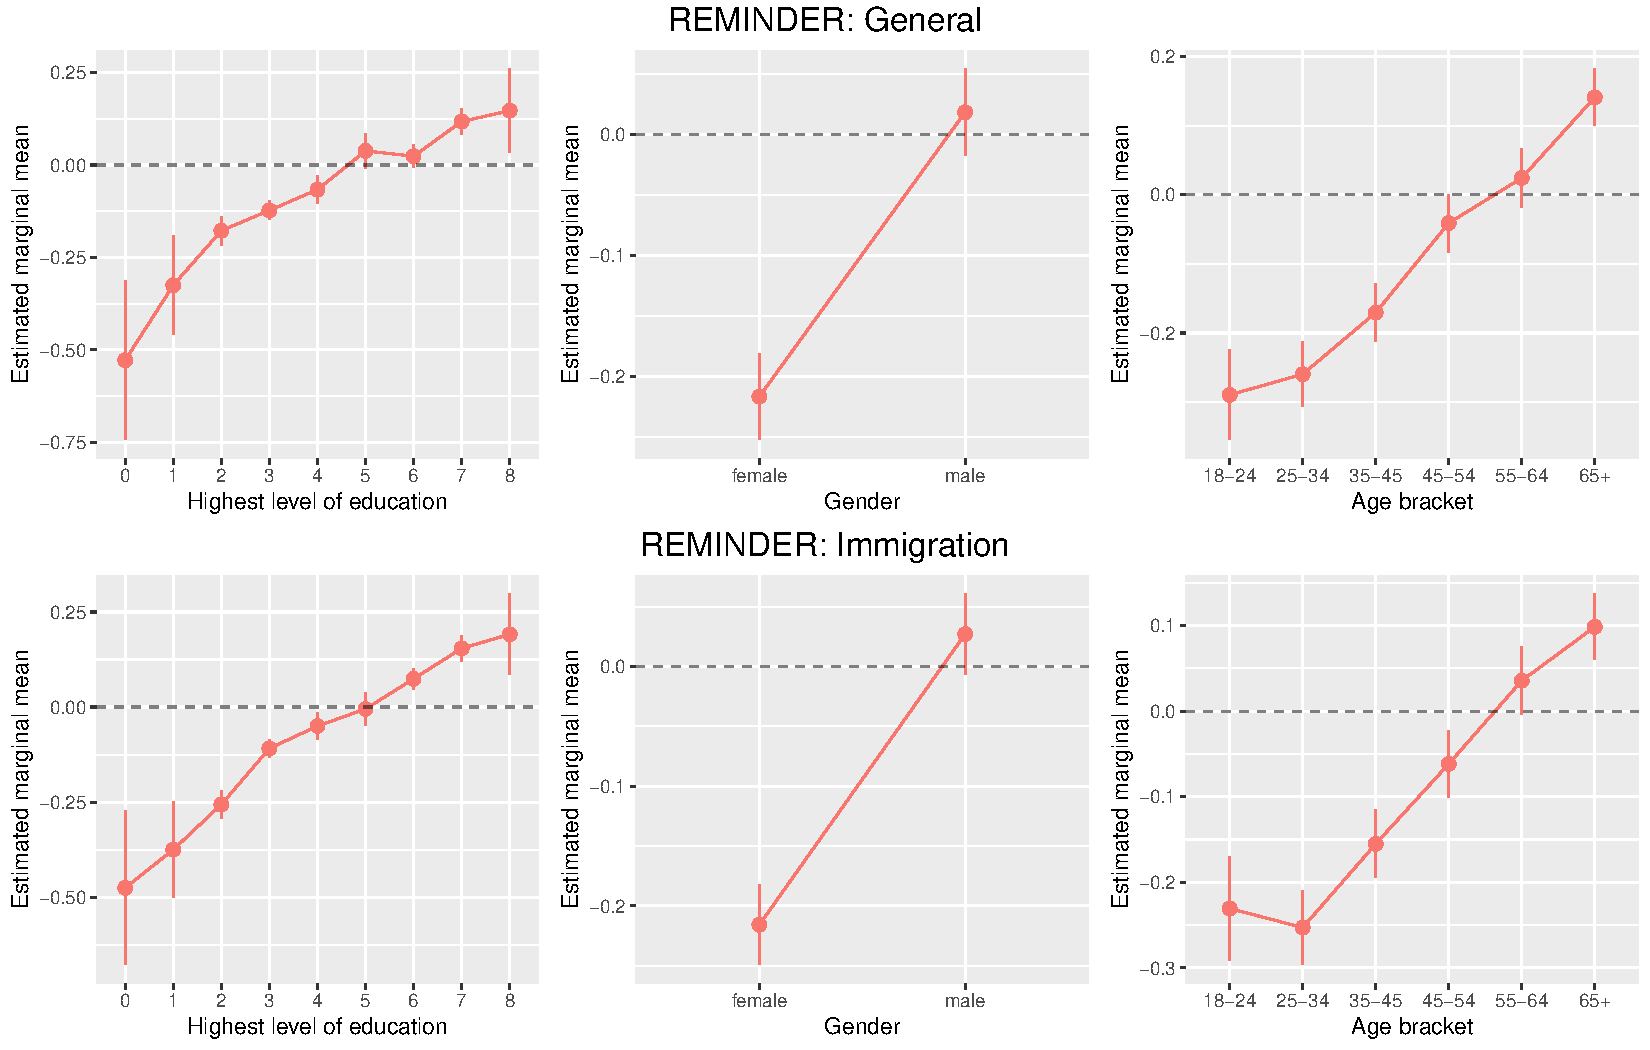
\includegraphics[width=1\linewidth]{Revisiting-the-Measurement-and-Dimensionality-of-Political-Knowledge--Evidence-from-Seven-European-Countries_files/figure-latex/emmeans_plots1-1} \caption{Estimated marginal means for REMINDER knowledge scales}\label{fig:emmeans_plots1}
\end{figure}

\begin{figure}[!h]
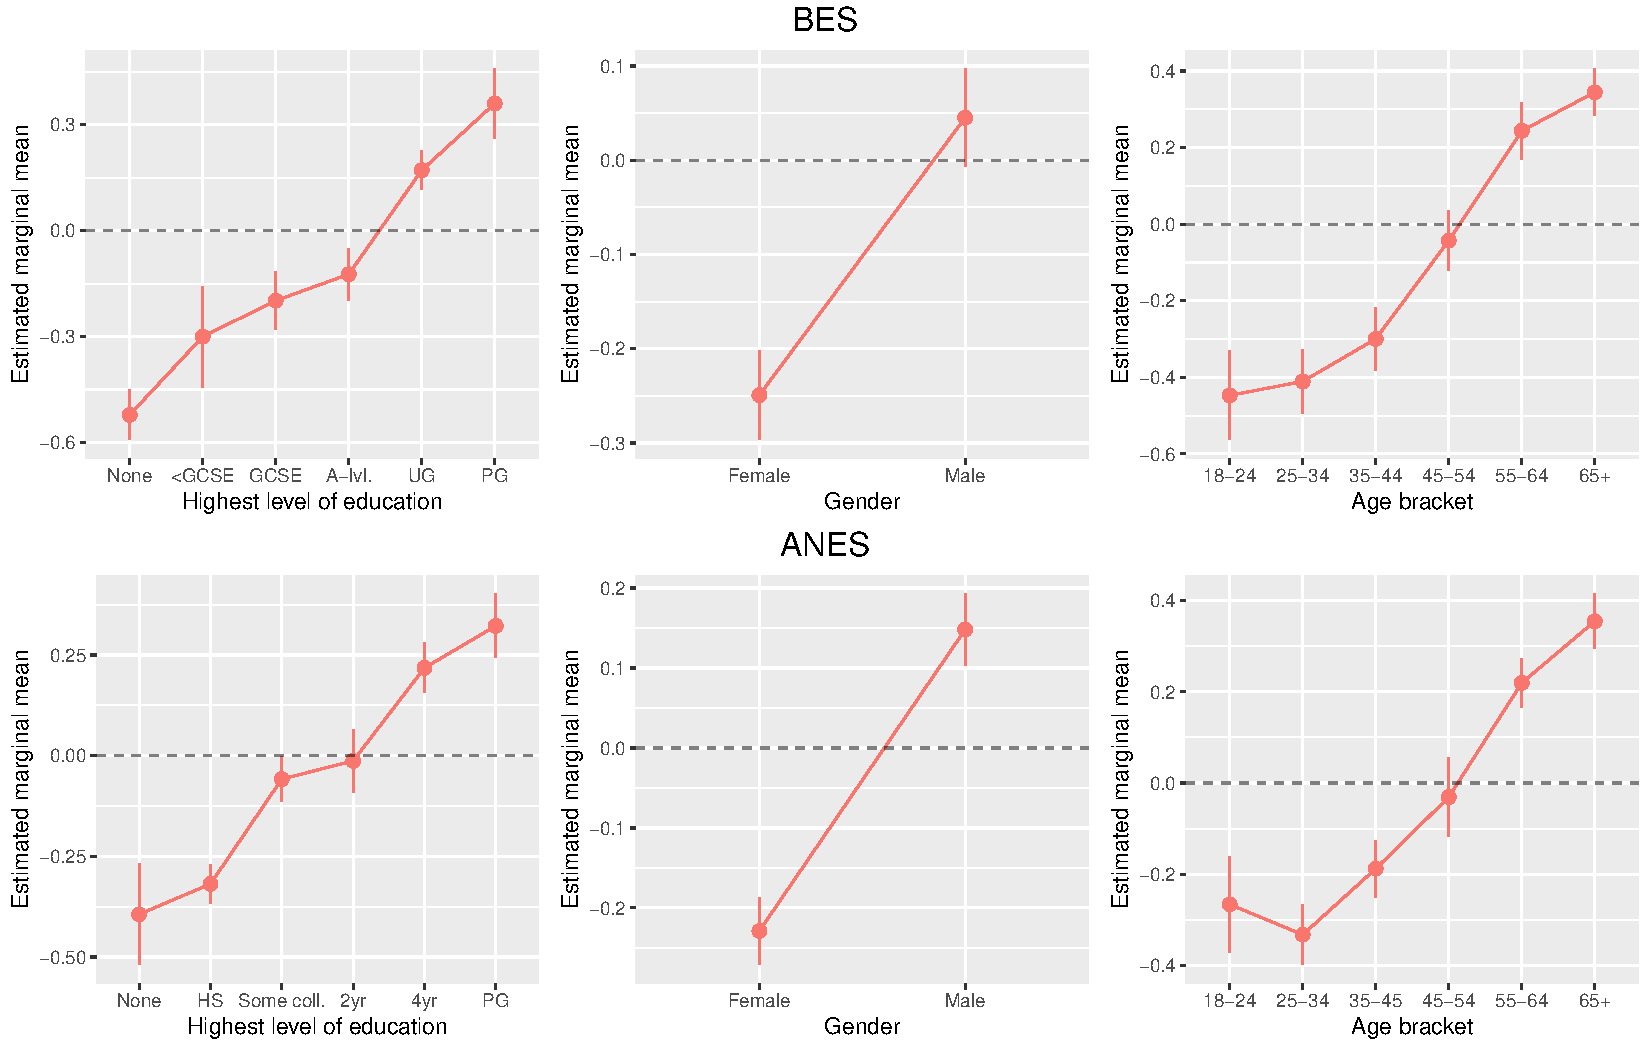
\includegraphics[width=1\linewidth]{Revisiting-the-Measurement-and-Dimensionality-of-Political-Knowledge--Evidence-from-Seven-European-Countries_files/figure-latex/emmeans_plots2-1} \caption{Estimated marginal means for BES and ANES knowledge scales}\label{fig:emmeans_plots2}
\end{figure}

Looking at Figure \ref{fig:emmeans_plots1} first, we can see that the
estimated marginal means for each of the three demographic variables are
very similar across the general and immigration specific knowledge
scales. This is consistent with the evidence from previous sections for
the generalist assumption -- if both scales tap into the same underlying
trait, then we should expect the marginal means to exhibit similar
patterns across these variables, as indeed they do. Turning then to
Figure \ref{fig:emmeans_plots2}, the fact that the two scales from the
previous figure moreover exhibit similar patterns in their marginal
means to the two established scales from BES and ANES offers further
evidence for both the generalist assumption, and for construct validity,
i.e., for the scales tapping into a form of knowledge in particular.

Breaking down the estimated means from the REMINDER scales by the seven
nationalities in the data set in Figures \ref{fig:emmeans_plots3a} and
\ref{fig:emmeans_plots3b}, we also see that, while the smaller sample
sizes render the results somewhat more noisy, the observations made in
relation to the aggregated data generally hold also in the case of the
individual countries as well. This offers some evidence that the
generalist assumption is robust in the face of geographical segmentation
as well.

\begin{figure}[!h]
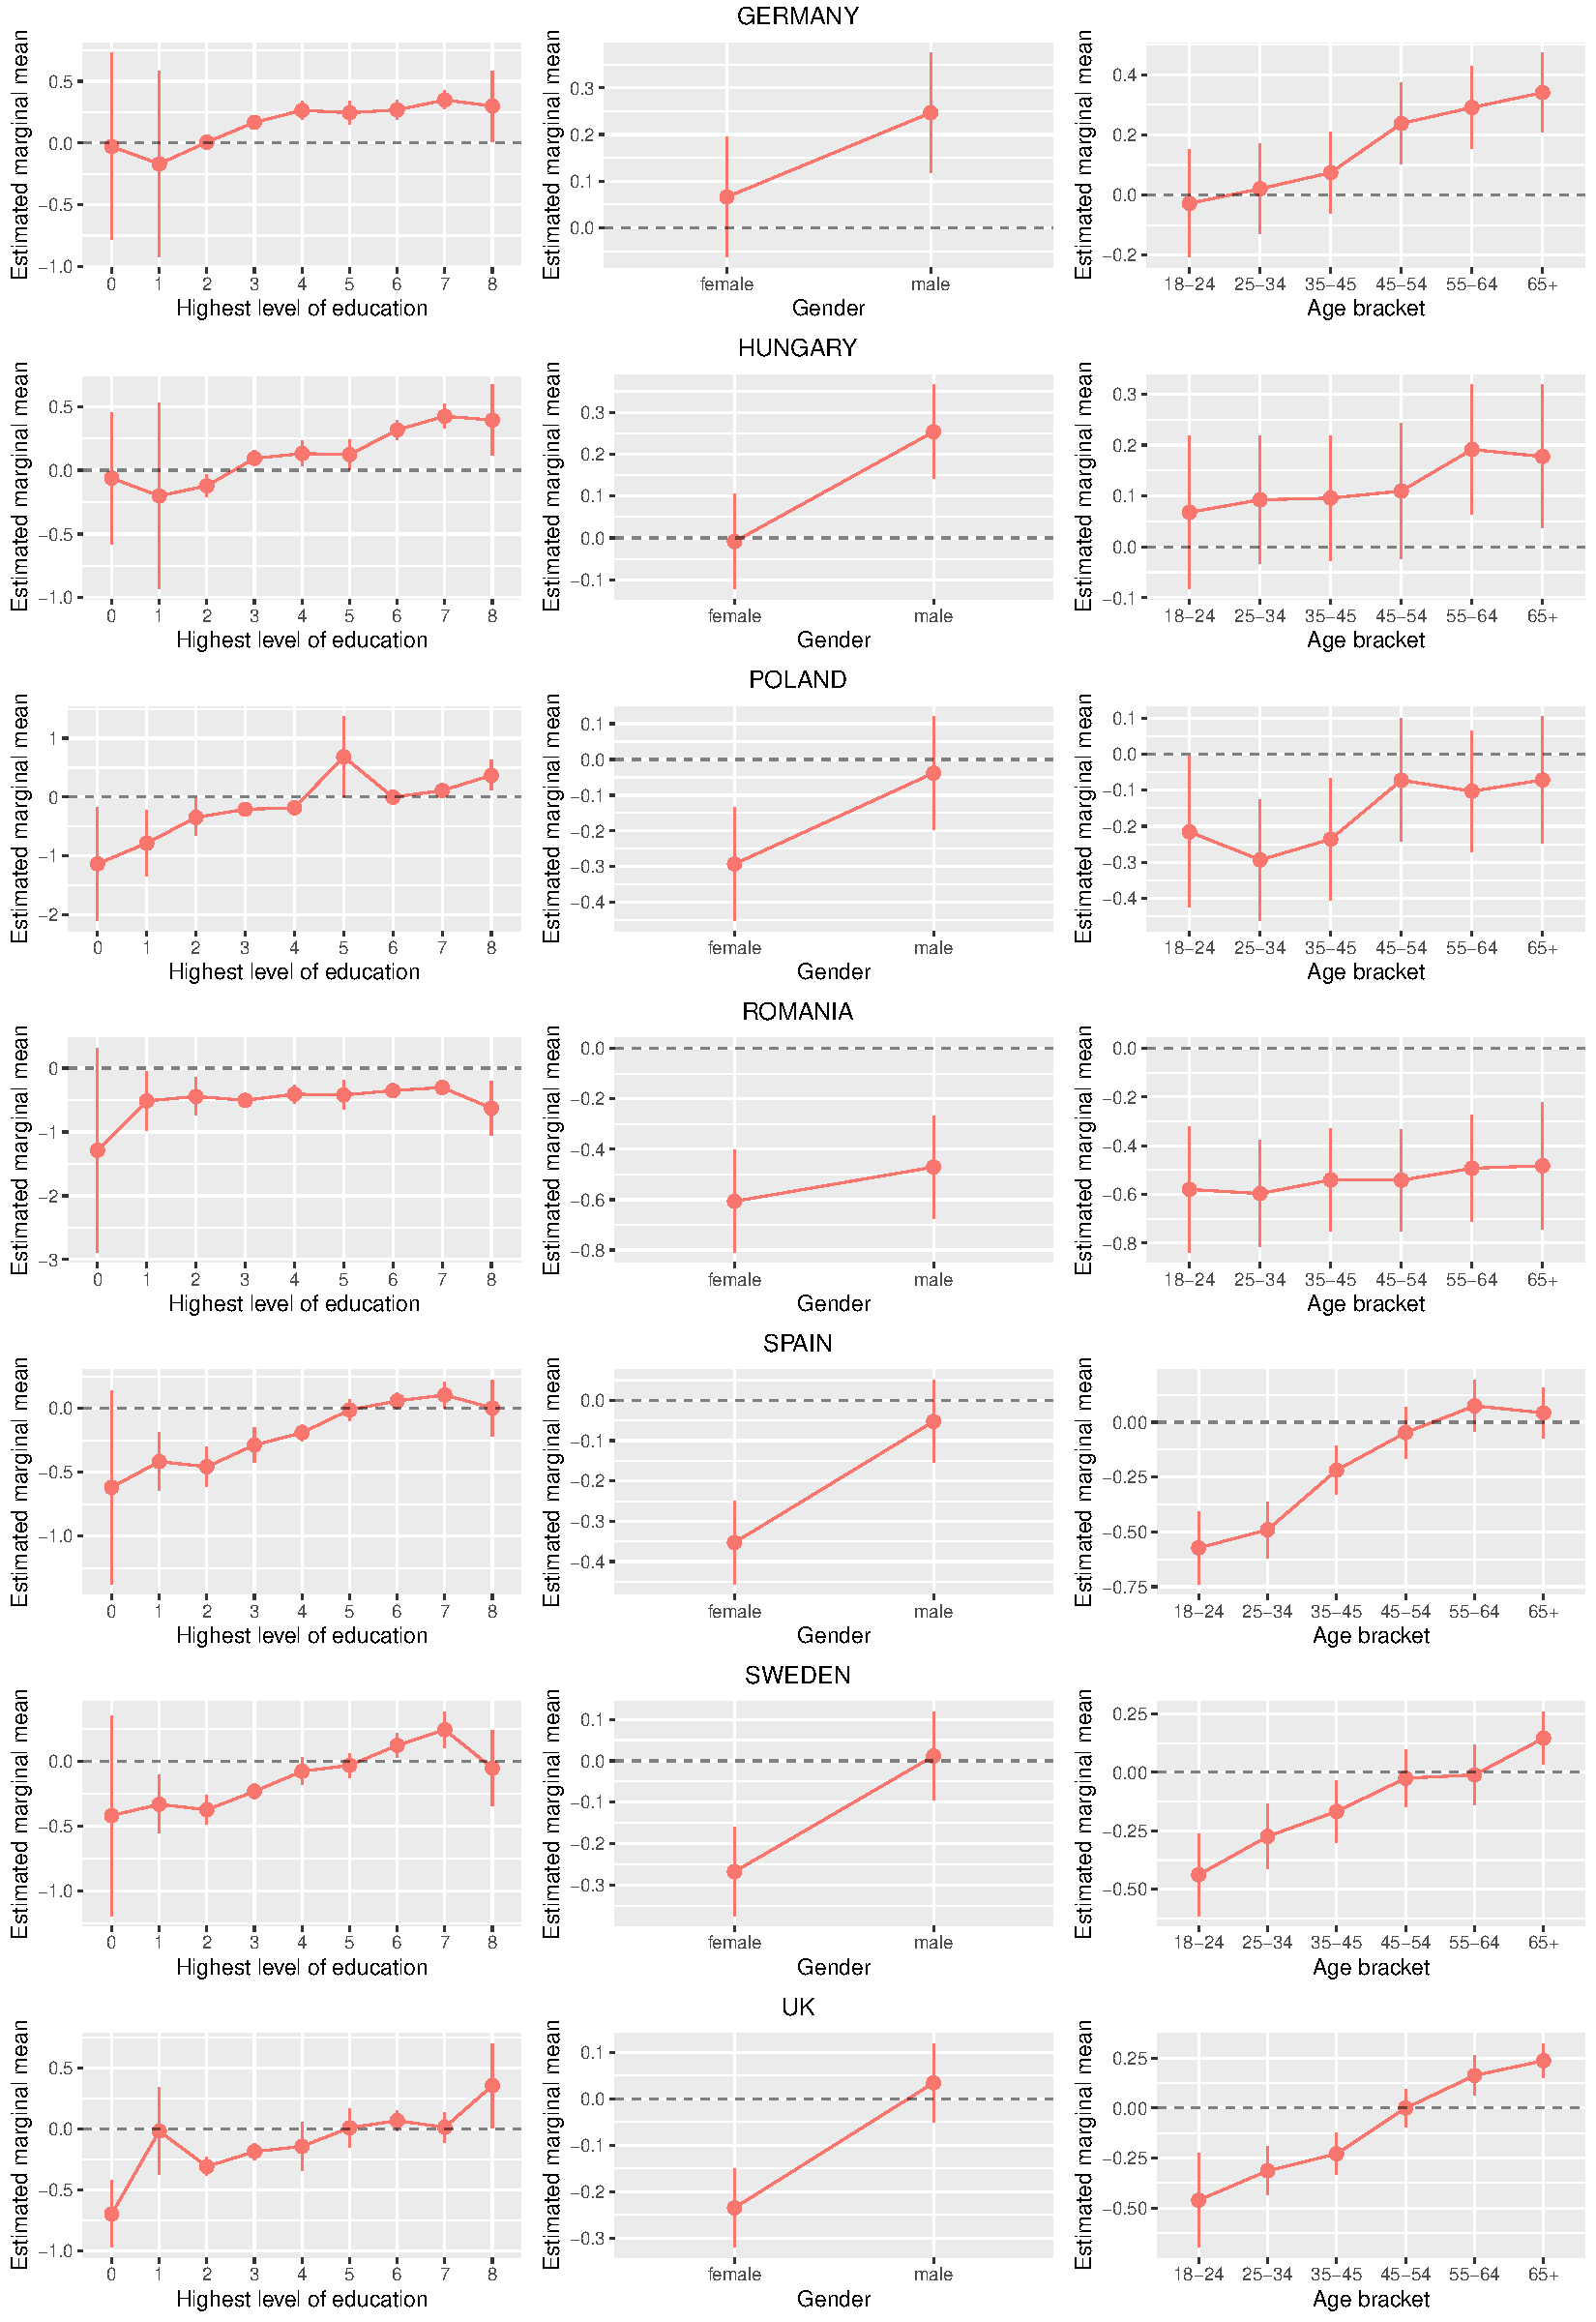
\includegraphics[width=1\linewidth]{Revisiting-the-Measurement-and-Dimensionality-of-Political-Knowledge--Evidence-from-Seven-European-Countries_files/figure-latex/emmeans_plots3a-1} \caption{Estimated marginal means for general knowledge scale by country}\label{fig:emmeans_plots3a}
\end{figure}

\begin{figure}[!h]
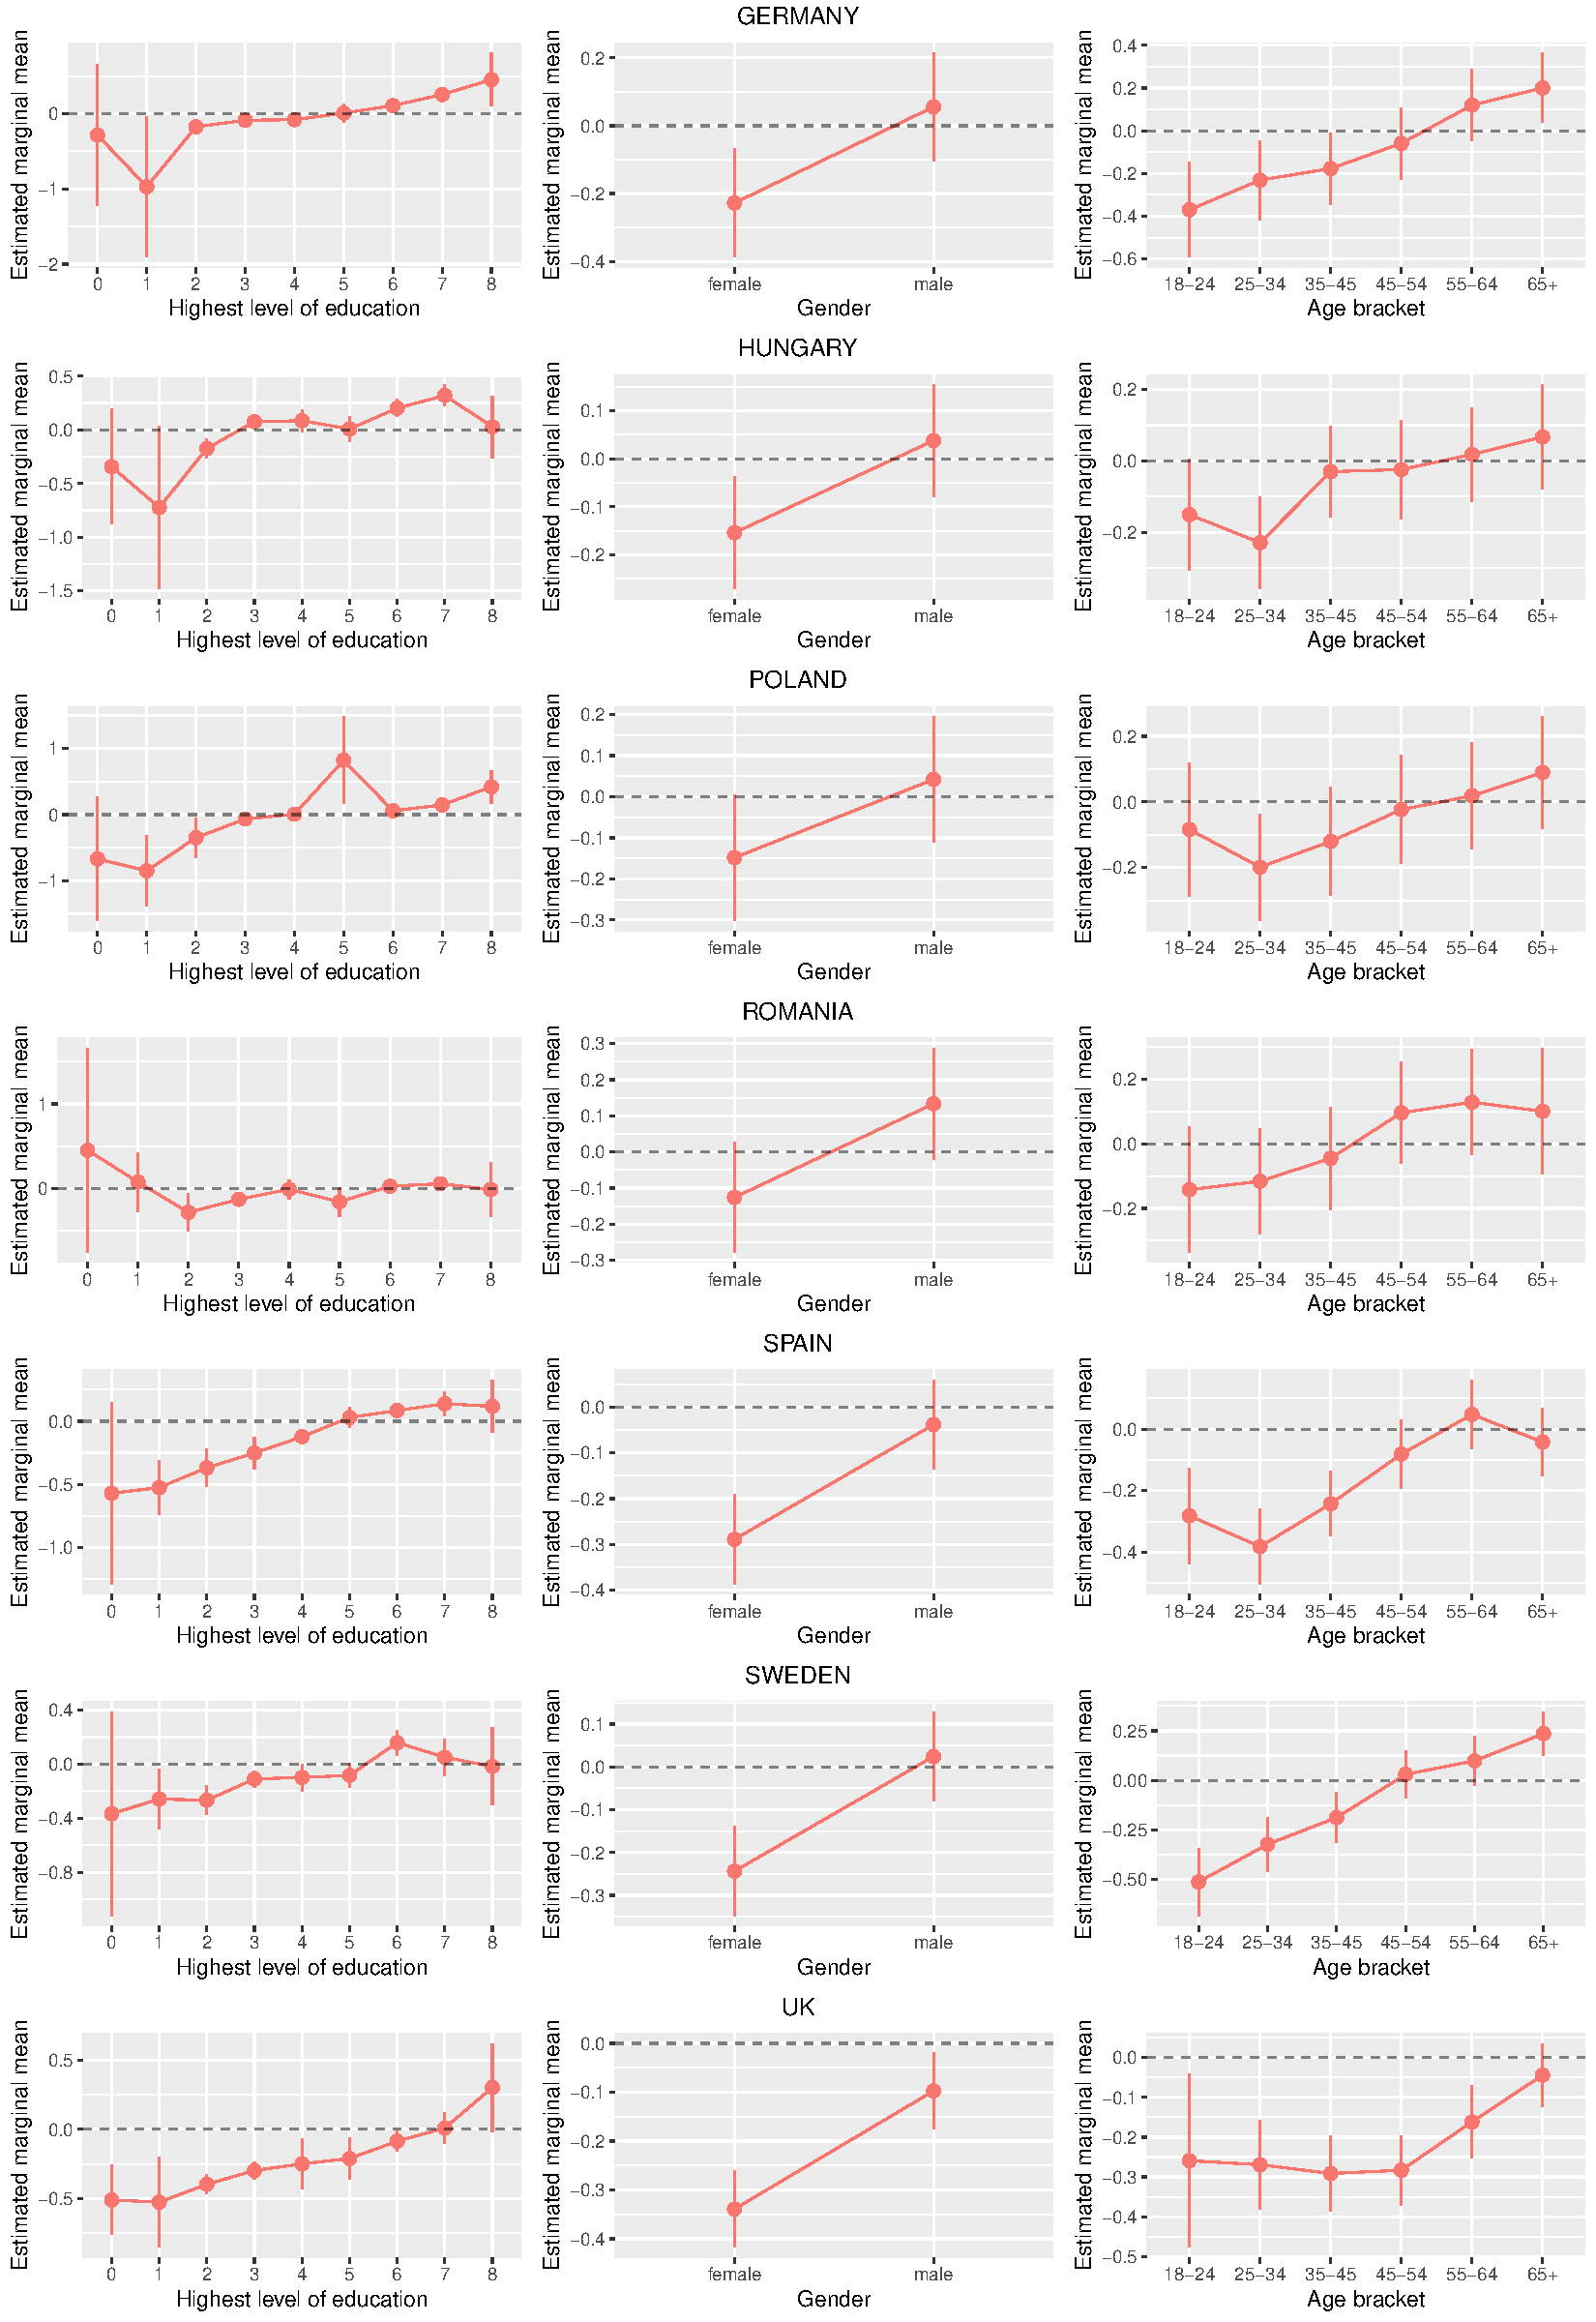
\includegraphics[width=1\linewidth]{Revisiting-the-Measurement-and-Dimensionality-of-Political-Knowledge--Evidence-from-Seven-European-Countries_files/figure-latex/emmeans_plots3b-1} \caption{Estimated marginal means for immigration knowledge scale by country}\label{fig:emmeans_plots3b}
\end{figure}

\hypertarget{step-3-stress-testing-the-generality-of-the-generalist-assumption}{%
\subsection{Step 3: Stress-testing the generality of the generalist
assumption}\label{step-3-stress-testing-the-generality-of-the-generalist-assumption}}

So far, we have seen evidence for the generalist assumption in the
context of general political knowledge versus immigration specific
knowledge. This evidence does not rule out that there is something
unique about immigration specific knowledge in particular, and that the
generalist assumption as such would not generalize to other,
issue-specific areas. For this reason, in our third and final step, we
compare the marginal means of our two scales to that of two, separate
issue-specific scales: one relating to public health, and to knowledge
about COVID in particular; and one relating to knowledge about climate
change.

Our COVID data set comes from a a pre-registered survey experiment (N =
2,917 UK citizens) fielded in the UK through the wake of its first wave
in July 2020 (Allen and Ahlstrom-Vij, under review). The survey contains
the following knowledge items, which together form a scale satisfying
standard assumptions for IRT:

\begin{quote}
(COV1) COVID-19 can be transmitted in areas with hot and humid climate
(true)\\
(COV2) There is currently no vaccine to protect against COVID-19 (true
{[}in July 2020{]})\\
(COV3) Most people who get COVID-19 recover from it (true)
\end{quote}

The climate change data set is from the European Perceptions of Climate
Change survey (Pidgeon 2016). The survey was not designed to measure
knowledge about climate change in particular, but it contains the
following three items which reasonably can be taken to tap into such
knowledge, and moreover also form a scale satisfying standard
assumptions for IRT:

\begin{quote}
(CC1) As far as you know, do you think the world's climate is changing
or not? (Correct: The climate is changing)\\
(CC2) Thinking about the causes of climate change, which, if any, of the
following best describes your opinion? (Correct: Climate change is
partly, mainly, or completely caused by human activity)\\
(CC3) To the best of your knowledge, what proportion of scientists agree
that climate change is happening and that humans are largely causing it?
(Correct: The vast majority of scientists agree, at 80\% or more)
\end{quote}

Figure \ref{fig:emmeans_plots4} plots the estimated means for the same
demographic variables as in the previous section for the above COVID and
Climate Change knowledge scales.

\begin{figure}[!h]
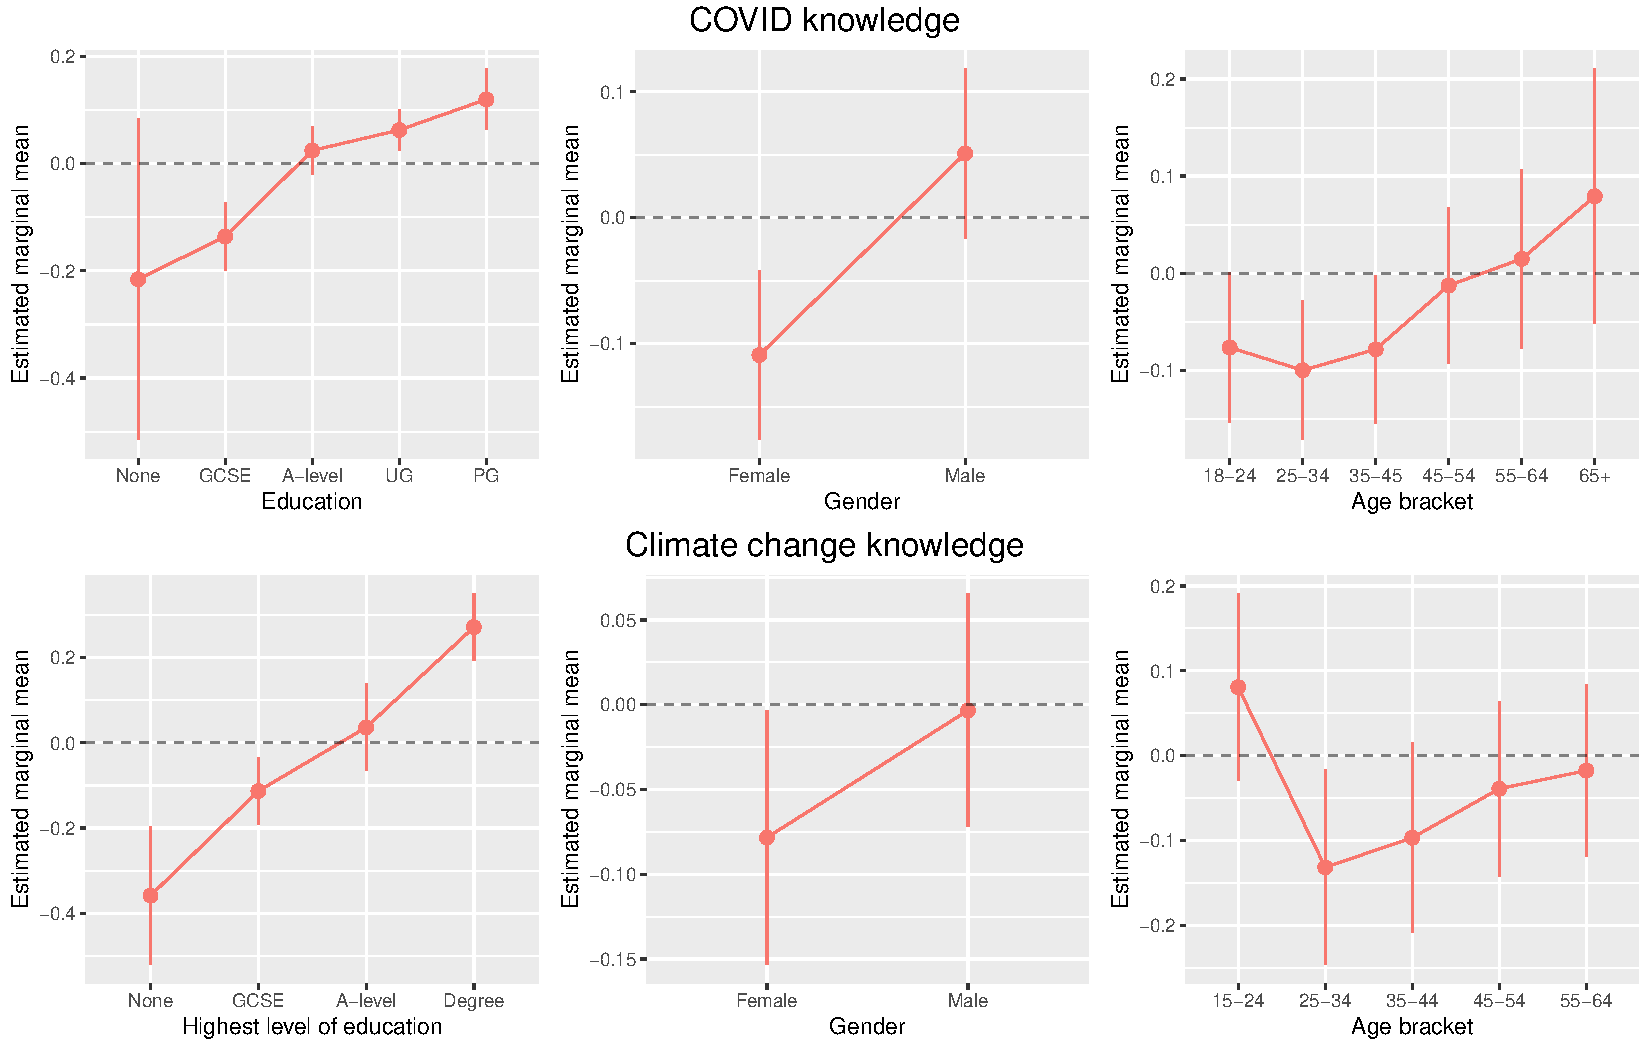
\includegraphics[width=1\linewidth]{Revisiting-the-Measurement-and-Dimensionality-of-Political-Knowledge--Evidence-from-Seven-European-Countries_files/figure-latex/emmeans_plots4-1} \caption{Estimated marginal means for COVID and Climate Change knowledge scales}\label{fig:emmeans_plots4}
\end{figure}

For both scales, the marginal means by education shows the same,
monotonic trend that we saw in both Figure \ref{fig:emmeans_plots1} and
\ref{fig:emmeans_plots2}. In the case of both scales, men also generally
have more knowledge than women, which again is in line with what we
found in regards to the scales in the previous section. In the case of
age, we see a much more pronounced drop from the first to the second
bracket than what we saw for our previous four scales. Additionally, the
climate change scale in particular exhibits a less straightforward
relationship than the other scales, in having substantially higher
levels of knowledge in the first bracket, and also a dip in the case of
the final bracket (65+). It is worth reflecting on whether knowledge
about climate change can be expected to have a non-traditional
distribution, especially given the potential for higher levels of
awareness among younger compared to older people, in light of how the
former have a greater number of years of exposure to the effects of
climate change ahead of them.

\hypertarget{guidance-for-researchers}{%
\section{Guidance for researchers}\label{guidance-for-researchers}}

We mentioned at the outset that one ambition with revisiting the
dimensionality of knowledge was to outline a series of steps that that
be replicated by others in need to of evaluating the dimensionality of
their knowledge scales(s). In light of that, and the steps taken as part
of our analysis above, we recommend the following:

\begin{enumerate}
\def\labelenumi{\arabic{enumi}.}
\tightlist
\item
  Start by conducting a parallel analysis on the total set of knowledge
  items, and then investigate the loadings from an exploratory factor
  analysis (EFA) on those same items.\\
\item
  Let your EFA inform a confirmatory factor analysis that compares a
  unidimensional model to one or several multi-dimensional models,
  depending on the number of factors suggested by the EFA, and in order
  to see whether the former exhibits a good enough fit to compete with
  the multi-dimensional model(s). If it can, this would count towards
  unidimensionality.\\
\item
  Construct two or more knowledge scales, depending on the
  dimensionality under investigation, and then use each scale as an
  outcome in a regression model, with gender, education, and age as
  predictors. See if there any similarities in coefficients between the
  two. High similarity would count towards unidimensionality.\\
\item
  Calculate marginal mean levels of knowledge by gender, education, and
  age, respectively for each of your scales, and compare the patterns in
  these levels to those exhibited in Figures \ref{fig:emmeans_plots1},
  \ref{fig:emmeans_plots2} and \ref{fig:emmeans_plots4}. Similarity with
  the patterns found ere would count towards unidimensionality.
\end{enumerate}

For any given project, all or only some of these steps will be
appropriate or possible. However, it is our hope that the above steps
will nonetheless offer helpful guidance for researchers concerned with
questions about the dimensionality of their knowledge scales.

\hypertarget{discussion}{%
\section{Discussion}\label{discussion}}

As research into the consequences of political knowledge demonstrates,
being more informed potentially matters not only for how people vote but
also what they think about specific issues. Whether on principled
grounds or simply for reasons of being limited to general knowledge
items in available data sets, however, the majority of existing work is
based on observational survey data and typically invokes what we have
called a generalist assumption: that knowing a great deal about general
political topics is indicative of having greater knowledge about
specific issues as well. Yet testing whether this is the case -- and in
which contexts -- is difficult owing to the lack of cross-national
survey instruments that combine both general and issue-specific
knowledge questions.

In response, we have exploited a recent large-scale survey that,
unusually, contains both types of items in one instrument across seven
European countries. Combining several analytical approaches, we conclude
that the preponderance of evidence points to the generalist assumption
being defensible. First, exploratory and confirmatory factor analyses
applied to various combinations of the knowledge items revealed how the
collection of questions performed well when treated unidimensionally.
Second, in terms of construct validity, key demographic features that
prior theory leads us to expect should matter exhibit very similar
associations between our political and immigration knowledge scales.
Moreover, both scales exhibit similar patterns in in estimated marginal
mean level of knowledge as established knowledge scales from the BES and
ANES, both in the aggregate and when broken down in terms of the seven
individual countries. Third, the same marginal means patterns arise also
in the case of other issue-specific knowledge scale, in relation to
public health (COVID) and climate change in particular, which offers
some reason to believe that the generalist assumption is robust across
individual issues, as opposed to holding for immigration knowledge only.

Our study has implications for the ways that researchers use political
knowledge questions as they study domain-specific attitudes and
preferences. Although we argue the generalist assumption is defensible,
at least in the particular domains that we have been concerned with in
this paper (i.e., immigration, public health, and climate change), we
also emphasize that it should not be deployed uncritically. Rather, we
advise that researcher should stress-test it as far as the available
data allow, notably by including knowledge items from different domains,
and by using a combination of methods to evaluate its plausibility in
specific contexts. To that end, and in the spirit of Open Science, we
also publicly offer our approach (its code and method) as a template for
others.\footnote{See https://github.com/ahlstromvij/REMINDER\_project
  for a repository containing all the code used in generating the
  analysis above.}

\hypertarget{references}{%
\section{References}\label{references}}

References forthcoming\ldots{}


\begin{notes}[Acknowledgements]
WA acknowledges support from the British Academy (grant number
PF21\textbackslash210066)
\end{notes}




\end{document}
